% Slug: four-of-diamonds
% Description: ?
% Author: Cisco
% Story: Cisco
% Test Data: Cisco
% Testers: ?
% Editorial: ?
% TempSlug: four-of-diamonds

% Please don't modify or delete TempSlug

\problem{Mixed Messages}
I have a puzzle for you!  Can you decipher the hidden meaning in the following message?
\begin{center}
    \texttt{4427777}
\end{center}
This is a classic cipher.  Here's a hint:
\begin{center}
    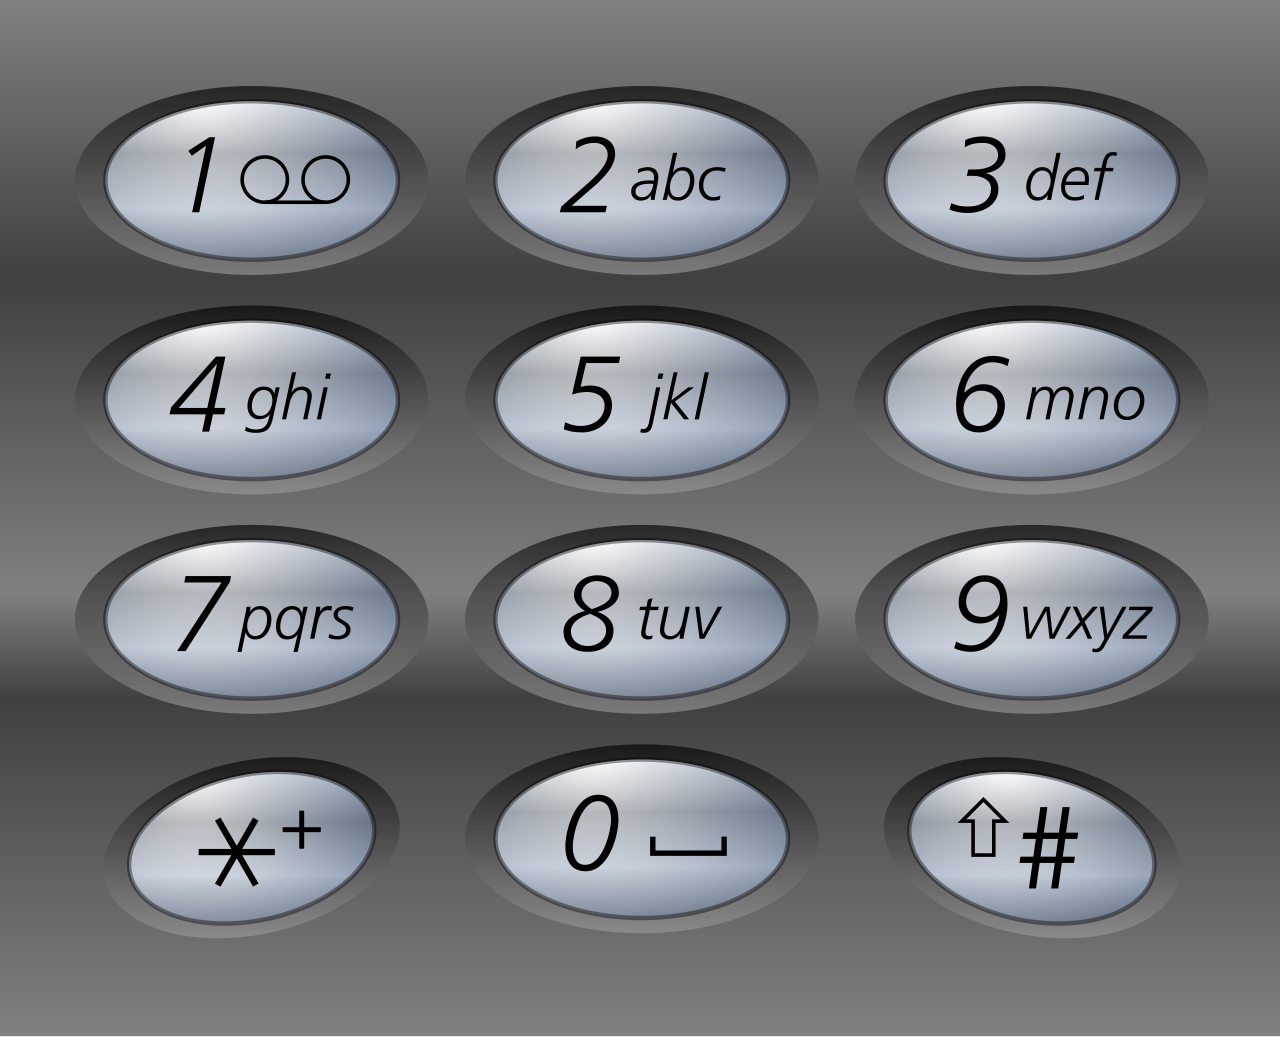
\includegraphics[width=0.25\linewidth]{img/keypad.png}

    \textit{Image taken from Wikipedia}
\end{center}
On an old cellphone keypad, letters are typed by pressing the corresponding key some number of times.  Each key is responsible for multiple letters (in the order they are written on the keypad), and each tap of the key would let you \textit{cycle} through your options which letter gets typed in.

For example, tapping \texttt{2} once would encode \texttt{a}, tapping it twice would encode \texttt{b}, and tapping it thrice would encode \texttt{c}.  One would ``lock in'' a choice by pausing before tapping again (usually you would have to wait for around one second between inputs).

We can use this to create a simple cipher.  Replace each English letter with the corresponding digit of the key it belongs to, repeated a number of times equal to the number of times you would tap that digit to get that letter.

For example, to translate the string \texttt{has}, we note that: \texttt{h} is \texttt{44}; \texttt{a} is \texttt{2}; and \texttt{s} is \texttt{7777}.  Concatenating them, we see that \texttt{has} is \texttt{4427777}.

The issue with this scheme is that by not encoding the pauses, it is posisble to have multiple words that map to the same ciphertext, making the message ambiguous.

For example, to translate the string \texttt{harp}, we note that: \texttt{h} is \texttt{44}; \texttt{a} is \texttt{2}; \texttt{r} is \texttt{777}; \newline and \texttt{p} is \texttt{7}.  Concatenating them, we see that \texttt{harp} is \textit{also} \texttt{4427777}.

Given a string of digits (each from \texttt{2} to \texttt{9}) to be interpreted as ciphertext, determine if the message is clear (if there is exactly one plaintext string which produces that ciphertext) or ambiguous (if multiple possible plaintext strings are encoded as that ciphertext).  \newline If the message is clear, please decode it for us as well!

\newpage

\subsection*{Input Format}

Input consists of a single line containing a string of digits (each from \texttt{2} to \texttt{9}), the ciphertext.

\subsection*{Output Format}

First, output a line containing either the string \texttt{CLEAR} or \texttt{AMBIGUOUS} according to the uniqueness of how to decode the ciphertext.

If \texttt{CLEAR}, also output another line containing the unique decrypted message (in all-lowercase letters).

\subsection*{Constraints}

\textit{Your program will only be tested on data that satisfies the following constraints.}

% Set to 10^5 in true bounds
\constraints{
    The ciphertext consists of at least $1$ and at most $100$ digits, each from \texttt{2} to \texttt{9}.\\
}

\textit{There is no need to validate in your program that these constraints hold.}

\subsection*{Sample I/O}

\begin{sampleIO}
\begin{verbatim}
725262
\end{verbatim}
&
\begin{verbatim}
CLEAR
pajama
\end{verbatim}
\end{sampleIO}

\begin{sampleIO}
\begin{verbatim}
4427777
\end{verbatim}
&
\begin{verbatim}
AMBIGUOUS
\end{verbatim}
\end{sampleIO}


% \subsection*{Explanation}
